\begin{figure}
    \centering
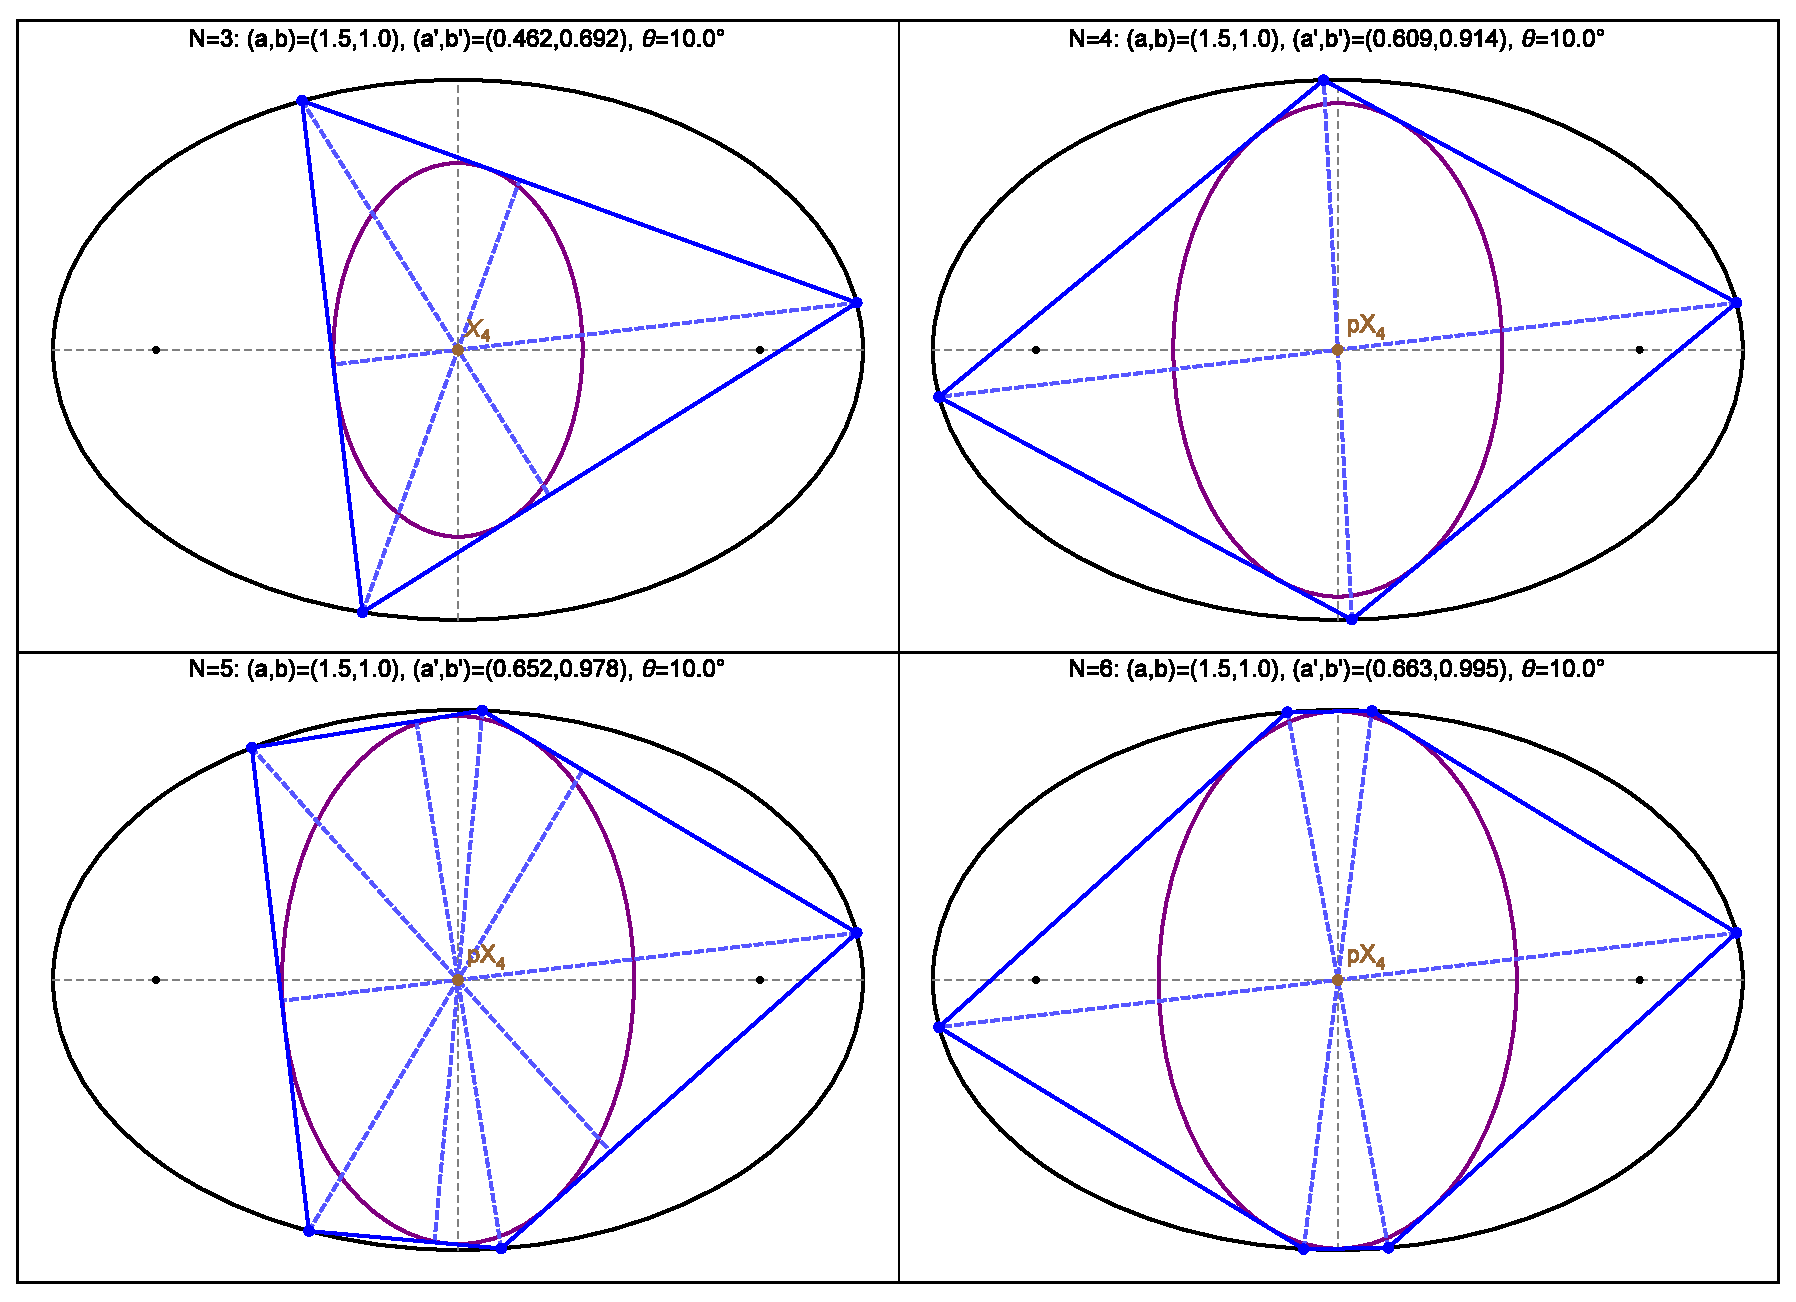
\includegraphics[width=\textwidth]{pics/0037_system_IV.eps}
    \caption{The dual Poncelet pair: the caustic (purple) is homothetic to the external ellipse rotated 90 degrees. N-Periodics are shown for N=3, 4, 5, and 6. For each case, the (pseudo)-altitudes meet at the common center.}
    \label{fig:dual}
\end{figure}

\begin{figure}
    \centering
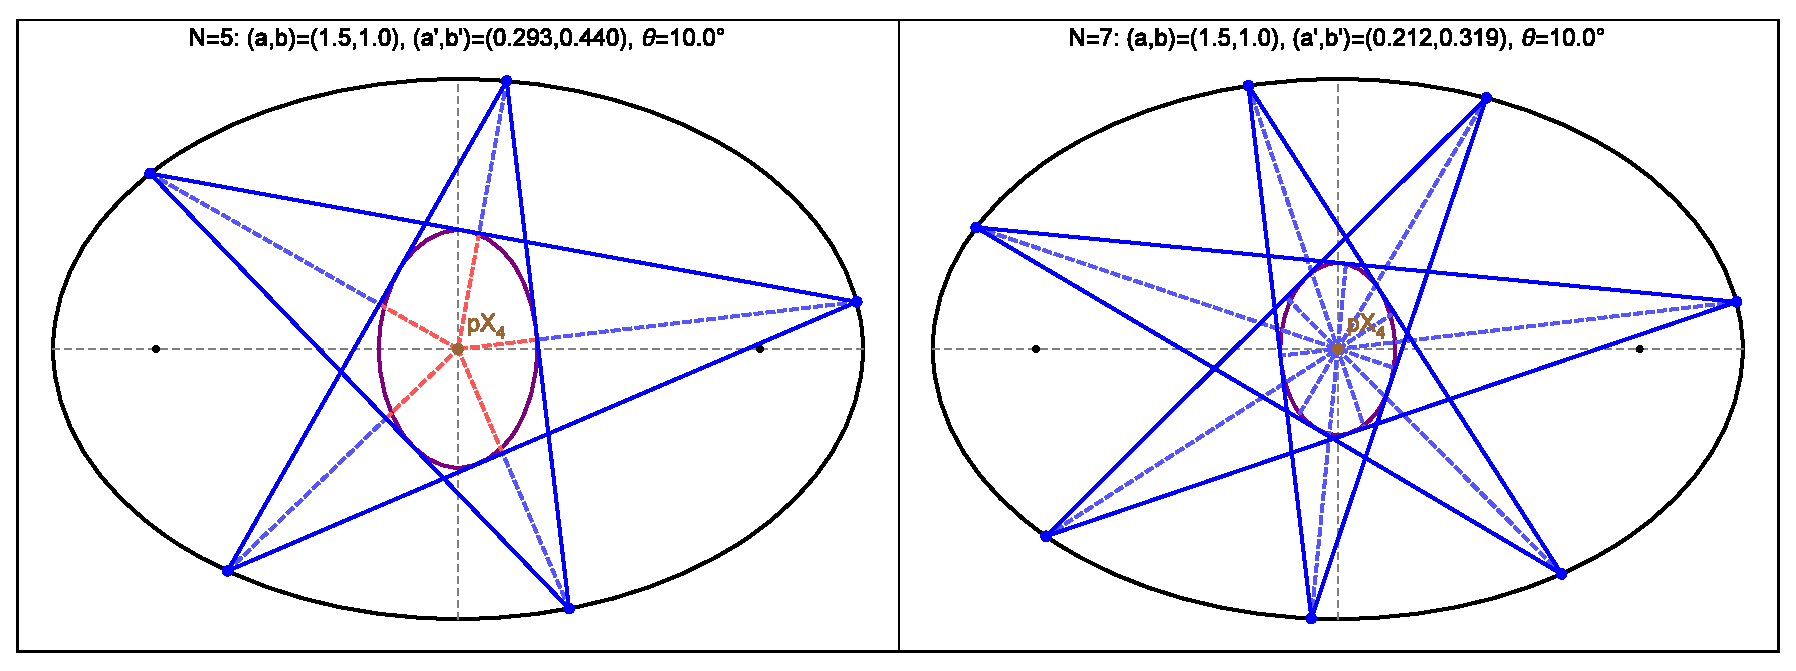
\includegraphics[width=\textwidth]{pics/0038_system_IV_star.eps}
    \caption{The dual Poncelet pair for self-intersecting 5- and 7-periodics. Their pseudo-altitudes also meet at the common center.}
    \label{fig:dual-star}
\end{figure}